\section{本章小结}
\label{sec:odeex-summary}

章首的三个方程分别暴露了三个问题：$\dot x=x^2$在有限时间内走不下去，$\dot x=2\sqrt{\lvert x\rvert}$有多条解，右端跳变的方程从零点出发无解。本章逐一给出了这些问题的条件，图~\ref{fig:odeex-summary-map}把它们串在一起。

局部存在只回答“有没有解”。有限维空间中右端连续就够了：Euler折线被关在盒子内，紧性抽出收敛的子列，连续性让极限满足方程。这条路线只给出一个解，子列的选择甚至依赖扰动，在无限维空间也可能失败。

唯一性回答“解是否由初值确定”。状态方向的局部Lipschitz条件使积分映射在短时间窗内成为压缩映射，靠完备性而不是紧性得到不动点，存在、唯一和迭代误差界同时得到。这一条件是便于验证的充分条件，单调性也能给出单向的唯一性；但Lipschitz常数对时间不局部可积时，唯一性可以失败。

\begin{BookInlineFigure}
  \centering
  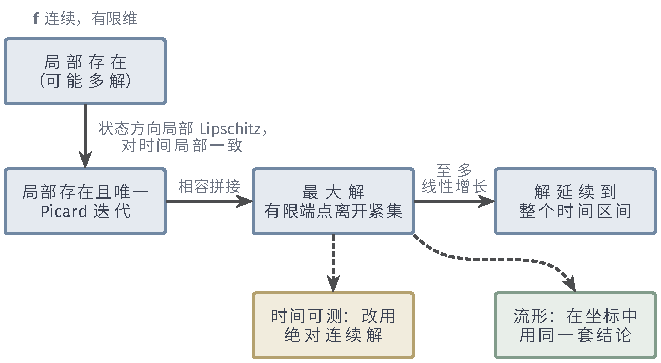
\includegraphics[width=112mm]{figures/06-differential-equations/01-ordinary-differential-equations/tikz/odeex-summary-map/figure.pdf}
  \caption{本章结论的依赖关系。从连续右端的局部存在出发，加上状态方向的局部Lipschitz条件得到局部存在且唯一，相容拼接得到最大解，至多线性增长使解延续到整个时间区间。虚线表示同一链条的两个推广：时间可测的方程和流形上的方程。}
  \label{fig:odeex-summary-map}
\end{BookInlineFigure}

最大延拓回答“局部解能接多长”。唯一性使局部解相容，并成唯一的最大解。解的定义区间是开区间，到有限端点时解离开定义域的每个紧集，表现为状态无界或趋近定义域的边界。全局存在回答“解能否走完给定的时间区间”，至多线性增长的右端保证了这一点，但解仍可能无界，全局存在也不提供唯一性。表~\ref{tab:odeex-summary}按问题列出了条件和反例。

\begin{BookInlineTable}
  \centering
  \caption{各问题的条件与反例}
  \label{tab:odeex-summary}
  \begin{tabularx}{\linewidth}{lXX}
    \toprule
    问题 & 条件（$\bm{f}$连续时） & 去掉条件的反例 \\
    \midrule
    局部存在 & 有限维，$\bm{f}$连续 & 右端跳变无解；$c_0$上连续而无解 \\
    唯一性 & 状态方向局部Lipschitz，对时间局部一致 & $2\sqrt{\lvert x\rvert}$的漏斗；系数$2/t$ \\
    最大延拓 & 局部存在且唯一 & 没有唯一性时最大解不唯一 \\
    全局存在 & 至多线性增长 & $\dot x=x^2$在$t=1$爆炸 \\
    \bottomrule
  \end{tabularx}
\end{BookInlineTable}

时间可测时，解要换成绝对连续解，对应的条件是：对时间可测、对状态连续、局部可积上界，由此得到存在；唯一性另要求状态方向的Lipschitz系数对时间局部可积，这不能由可测性或增长控制推出。这些结论只针对满足积分方程的绝对连续曲线，连续且几乎处处满足方程还不够，Cantor函数就是反例。

流形上，局部存在唯一性在每张坐标图内应用，切向量的变换规律使不同的图描述同一条曲线，Hausdorff条件和唯一性把它们接成最大积分曲线。坐标方程的爆炸可能只是走出了一张图，紧流形上的积分曲线对所有时间存在。切向条件和唯一性共同使解保持在流形上，测地线方程是这一结构的代表。

这些结论都只说明解的存在、唯一和存在区间，是有限时间上的定性结论。解对初值和参数怎样变化，变化能否求导，由第~\ref{chap:ode-sensitivity}章在这里的存在性保证上继续建立；第~\ref{chap:ode-numerical-methods}章的数值方法也是在解存在且唯一时才有明确的逼近目标。
